\documentclass[aspectratio=169]{beamer}%设置宽高比为16:9
\usepackage{graphicx} % 允许包含图像
\usepackage{booktabs} % 允许在表中使用\toprule、\ midrule和\ bottomrule
\usepackage{amsmath}
\usepackage{physics}
\usepackage[]{subcaption}
\usepackage[]{wrapfig}
\usepackage{tikz}
\usepackage{tikzducks}
\usetheme{Darmstadt}
\usepackage[]{bbding}
\usecolortheme{default}

\AtBeginSection[]{
	\begin{frame}
		\tableofcontents[currentsection]
	\end{frame}
} % 每到新的一节(Section)显示大纲

\title{The CHY Formalism for Massless Scattering}
\author[Author names]{%
		\textbf{Author: } 
		Bufan Zheng\\
		\textbf{Advisor: } 
		Yi-jian Du
}

\institute[WHU] % 您的机构将出现在每张幻灯片的底部,可能是节省空间的简写
{
	Wuhan University\\ % 你所在的机构
	\medskip
	\textit{whuzbf@qq.com}\Envelope\\ % Your email address
	\medskip
	\url{https://whuzbf.github.io}
	
}
\date{June 27, 2024} % 日期,可以更改为自定义日期
\begin{document}
	\begin{frame}
		\titlepage % 将标题页打印为第一张幻灯片
	\end{frame}
	
	\begin{frame}
		\frametitle{Overview} % 目录幻灯片
		\tableofcontents 
	\end{frame}
	\section{Scattering Amplitudes}
	\begin{frame}
		\frametitle{Feynman Diagrams}
		\begin{columns}
			\column{0.7\textwidth}
			\begin{itemize}
				\setlength{\itemsep}{.3cm}
				\item <1-> {
					For \textbf{QED} process, Feynman diagram is a efficient tool to calculate scattering amplitudes.
				}
				\item <2-> {
					Feynman's rule is derived from the Lagrangian, there are many terms in the Lagrangian that are blame to \textbf{gauge redundancy}, which inevitably leads to very complex expressions for individual Feynman diagrams, but the superposition of all Feynman diagrams is simple.
					
					$$
					S_{\text{EH}}=\int d^{D}x\left[h\partial^{2}h+\kappa h^{2}\partial^{2}h+\kappa^{2}h^{3}\partial^{2}h+\kappa^{3}h^{4}\partial^{2}h+\cdots\right]
					$$
					% 比如说EH就因为规范冗余要带来无穷多的费曼图顶点项 %
				}
				\item <3-> {
					We have too many Feynman diagrams to sum. The number of diagrams is growing much \textbf{faster} than $n!$.
				}
			\end{itemize}
			\column{0.3\textwidth}
			\only <1,2> { %only和onslide的区别就是他不显示的时候不会占位% 
			\begin{figure}
				\centering
				% Requires \usepackage{graphicx}
				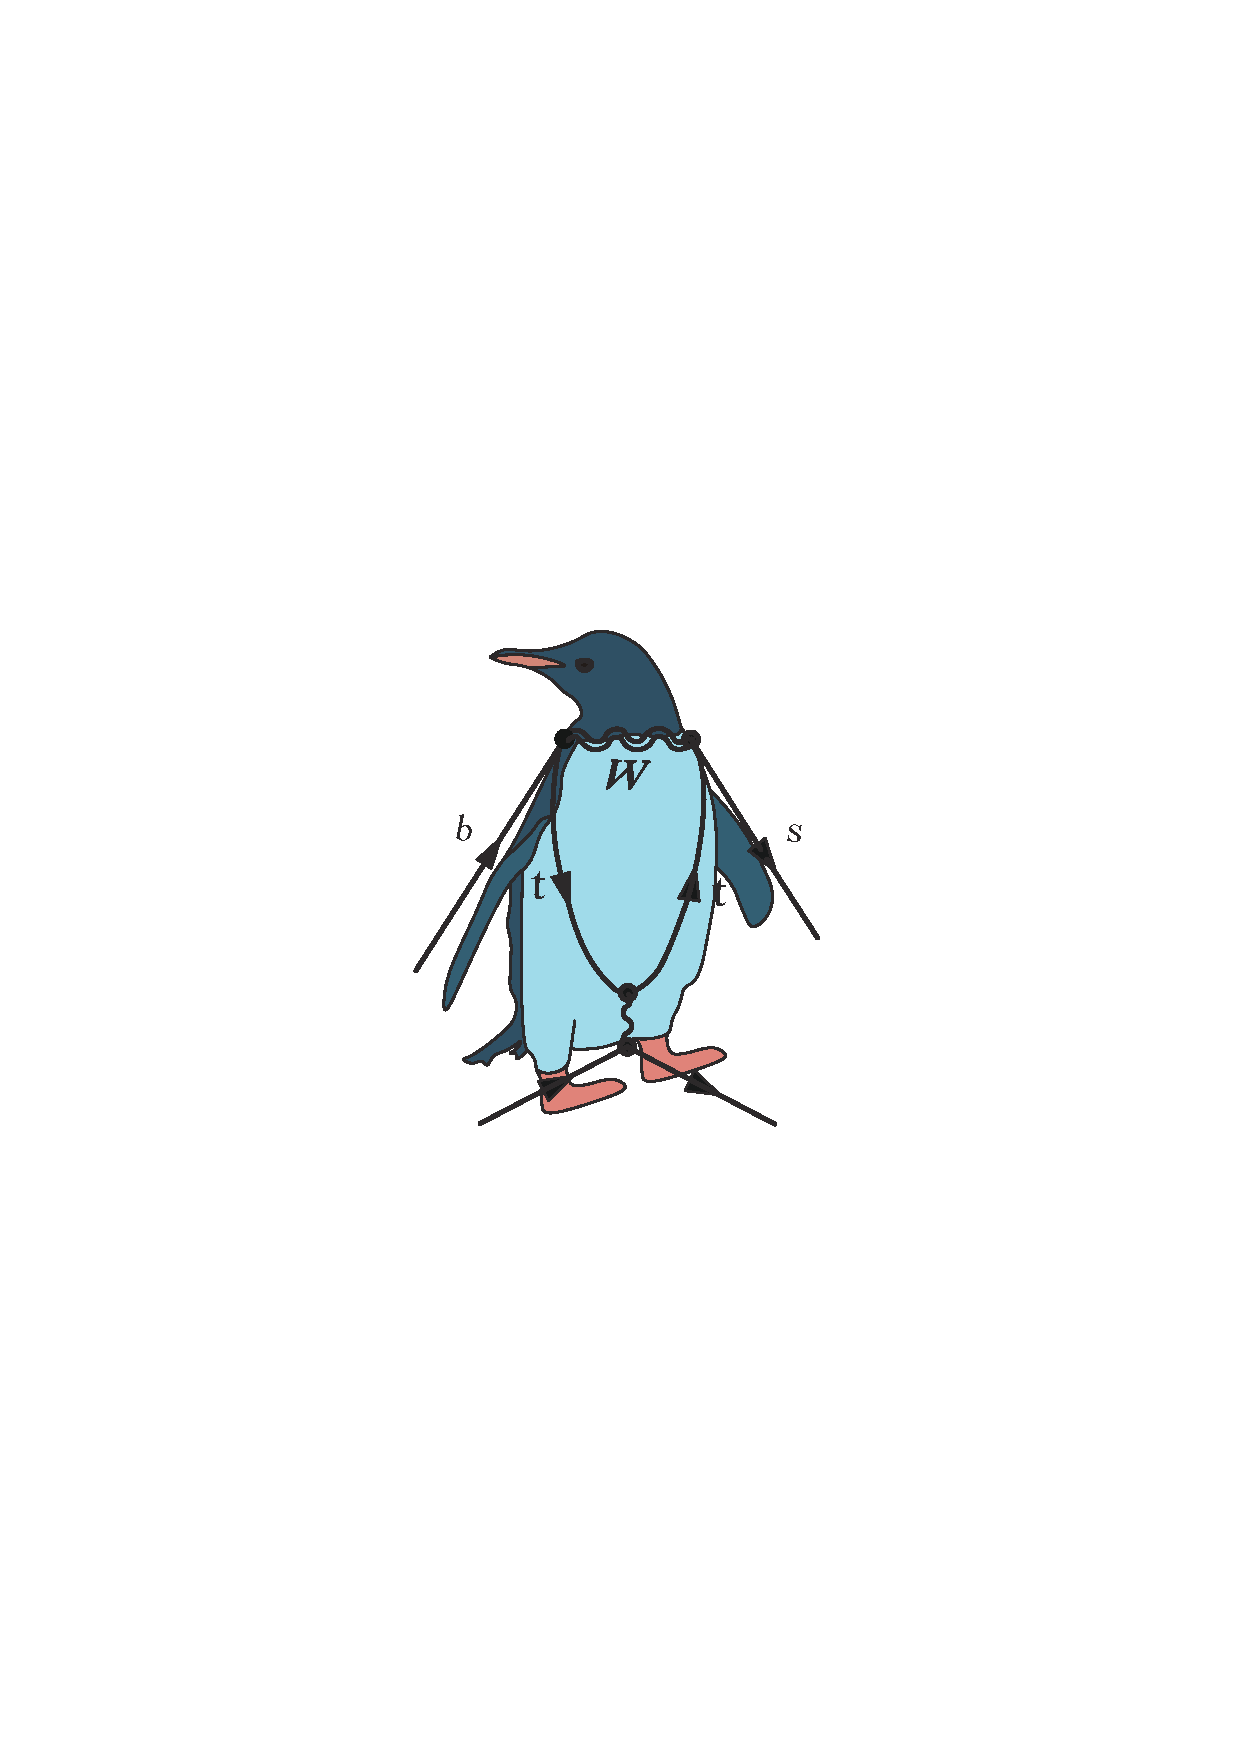
\includegraphics[width=4cm]{figs/penguin.pdf}
				\caption{Kawaii feynman diagram}
			\end{figure}}
			\only <3> {
				\begin{figure}
					\centering
					% Requires \usepackage{graphicx}
					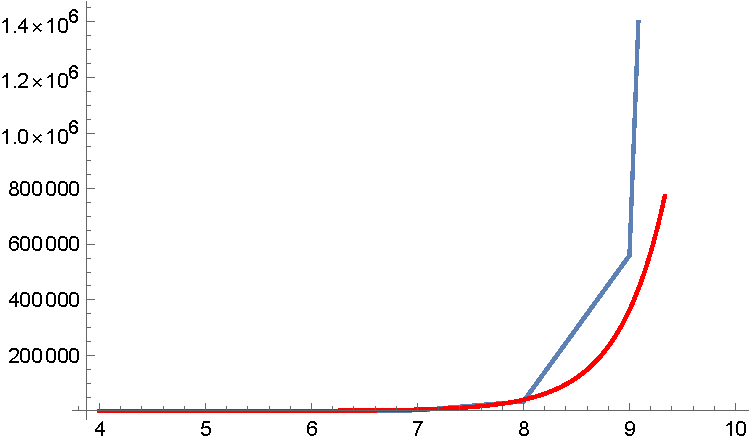
\includegraphics[width=4cm]{figs/2.pdf}
					\caption{Too many diagrams to sum}
			\end{figure}}
		\end{columns}
	\end{frame}
	\begin{frame}
		\frametitle{Chinese Magic}
		Spinor-Helicity Formalism
		\begin{itemize}
			\item {Using On-shell condition $p^2=0$:
			$$	
		    p_{a\dot{a}}=\sigma^\mu_{a\dot{a}}p_\mu=\lambda_a\tilde\lambda_{\dot{a}}\equiv|p]\bra{p}
			$$
			%这里的lambda就是wyle旋量其实% 
			we can do the same thing for $\bar \sigma^\mu_{\dot{a}a}p_\mu$ to define $\ket{p}$ and $[p|$.
			}
			
			\item {It is easy to see that $\ket{\cdot}$ and $|\cdot]$ automatically satisfy the gauge invariant condition:
				$$
				p^{\dot{a}b}|p]_b=0,\quad p_{a\dot{b}}|p\rangle^{\dot{b}}=0,\quad[p|^bp_{b\dot{a}}=0,\quad\langle p|_{\dot{b}}p^{\dot{b}a}=0.
				$$
			}
			
			\item {In fact we can use gauge degree of freedom to simplify our expressions:
				$$
				\epsilon_{\mu}^{+}(k;q)=\frac{\langle q^{-}|\gamma_{\mu}|k^{-}]}{\sqrt{2}\langle qk\rangle}
				$$
				The reference momenta $q$ can be chosen freely.
			}
		\end{itemize}
	\end{frame}
	
	\begin{frame}
		\frametitle{Tree Amplitudes of YM}
		\begin{itemize}
			\item {		
				MHV Amplitudes (Park-Taylor):
				$$
					A_n\left[1^+\ldots i^-\ldots j^-\ldots n^+\right]=\frac{\langle ij\rangle^4}{\langle12\rangle\langle23\rangle\cdots\langle n1\rangle}
				$$
		}
		\item{
			$\text{N}^k$MHV Amplitudes:
			$$
			\begin{aligned}A_n^{\mathrm{NPMHV}}(c_0,c_1,\ldots,c_p,n)&=\frac{\delta^{(4)}(p)}{\langle12\rangle\langle23\rangle\ldots\langle n1\rangle}\times\\&\times\sum_{\text{all paths of length }p}1\cdot\tilde{R}_{n;a_1b_1}\cdot\tilde{R}_{n;\{I_2\};a_2b_2}^{\{L_2\};\{U_2\}}\cdot\ldots\cdot\tilde{R}_{n;\{I_p\};a_pb_p}^{\{L_p\};\{U_p\}}\\
			&\times\left(\det\Xi_n^{\mathrm{path}}(c_0,\ldots,c_p)\right)^4\end{aligned}
			$$
			Complex, but fully solvable by computers
		}
		\end{itemize}
		% 有很多拉格朗日量本身看不出来的新性质,所以很值得做 %
	\end{frame}
	\section{scattering Equations}
	
	\begin{frame}
		\frametitle{Rimann Sphere}
		Momentum Space
		\begin{equation}
			\mathfrak{K}_{D,n}:=\{(k_1^\mu,k_2^\mu,\ldots,k_n^\mu)|\sum_{a=1}^nk_a^\mu=0,k_1^2=k_2^2=\cdots=k_n^2=0\}/SO(1,D-1)
		\end{equation}
		If there is no codimensional singularity
		\begin{equation}
			s_{a_1,a_2,...,a_r}:=(k_{a_1}+k_{a_2}+\cdots+k_{a_r})^2\neq 0,\quad \forall r=1,\ldots,n
		\end{equation}
		We can consider the moduli space of Riemann spheres $\mathbb{CP}^1$ with n distinct punctures on it to carve $\mathfrak{K}_{D,n}$ equivalently.
	\begin{equation}
		\label{3}
		\begin{gathered}
				\mathfrak{M}_{0,n}\equiv \{\sigma_1,\sigma_2,\ldots,\sigma_n\}/ SL(2,\mathbb{C})\\
			\mathfrak{K}_{D,n}\iff \mathfrak{K}_{D,n} \text{~by~} k_a^\mu=\frac1{2\pi i}\oint_{|z-\sigma_a|=\epsilon}dz\frac{p^\mu(z)}{\prod_{b=1}^n(z-\sigma_b)}
		\end{gathered}
	\end{equation}
	\end{frame}
	
	\begin{frame}
		\frametitle{Scattering Equations}
		Using eq.\ref{3}, we can derive the scattering equation:
		\begin{equation}
			\boxed{
				\sum_{b\neq a}\frac{s_{ab}}{\sigma_a-\sigma_b},\quad a={1,2,\ldots,n},\quad s_{ab}=2k_a\cdot k_b
			}
		\end{equation}
		\begin{itemize}
			\item<1-> {$n$ equations but only $n-3$ of them are independent.}
			\item<2-> {$(n-3)!$ solutions (codimensional singularity will bring degeneration).}
			\item<3-> {KLT orthogonality of solutions to scattering equations.
			\only<3>{
			\begin{equation}
				\label{5}
					\frac{(i,j)}{(i,i)^{\frac12}(j,j)^{\frac12}}=\delta_{ij}
			\end{equation}
		Where,
		$$(i,j):=\sum_{\alpha,\beta\in S_{n-3}}V^{(i)}(\alpha)S[\alpha|\beta]U^{(j)}(\beta)$$
		}
		
		\only<4>{
			Where,
			\begin{equation*}
				\begin{aligned}V(\omega)&=\frac1{(\sigma_1-\sigma_{\omega(2)})(\sigma_{\omega(2)}-\sigma_{\omega(3)})\cdots(\sigma_{\omega(n-2)}-\sigma_{n-1})(\sigma_{n-1}-\sigma_n)(\sigma_n-\sigma_1)},\\U(\omega)&=\frac1{(\sigma_1-\sigma_{\omega(2)})(\sigma_{\omega(2)}-\sigma_{\omega(3)})\cdots(\sigma_{\omega(n-2)}-\sigma_n)(\sigma_n-\sigma_{n-1})(\sigma_{n-1}-\sigma_1)}.\end{aligned}
			\end{equation*}}
			}
		\end{itemize}
	\end{frame}
	\section{CHY formalism}
	\setcounter{equation}{5}
	\begin{frame}
		\frametitle{Bi-adjoint Scalar, YM and Einstein Gravity}
		%最早论文提出的%
	    The amplitudes of many QFTs (at the tree level) can be expressed by a unified formula (Cachazo, He, Yuan, 2013).
		\begin{equation}
			\label{6}
				\boxed{
					\mathcal{A}_n=\int d\mu_n\mathcal{I}_n,\quad d\mu_n=\frac{d^n\sigma}{\text{volSL}(2,\mathbb{C})}\prod_a{'}\delta\bigg(\sum_{b\neq a}\frac{s_{ab}}{\sigma_{ab}}\bigg)
				}
		\end{equation}
		For different theories, the integral measure is the same, differing only in the CHY integrands $\mathcal{I}_n$
		\begin{equation}
			\mathcal{M}_n^{(\mathbf{s})}=\int\frac{d^n\sigma}{\text{vol}\operatorname{SL}(2,\mathbb{C})}\prod_a'\delta(\sum_{b\neq a}\frac{s_{ab}}{\sigma_a-\sigma_b})\left(\frac{\operatorname{Tr}(T^{\mathbf{a}_1}T^{\mathbf{a}_2}\cdots T^{\mathbf{a}_n})}{(\sigma_1-\sigma_2)\cdots(\sigma_n-\sigma_1)}+\ldots\right)^{2-\mathbf{s}}\left(\operatorname{Pf}'\Psi\right)^\mathbf{s}
		\end{equation}
		\only<1>{
			For Scalar, $s=0$,
			\begin{equation}
				\mathcal{L}^{\Phi^{3}}:=-\frac{1}{2}\partial_{\mu}\Phi_{I,\tilde{I}}\partial^{\mu}\Phi^{I,\tilde{I}}-\frac{\lambda}{3!}f_{I,J,K}\tilde{f}_{\tilde{I},\tilde{J},\tilde{K}}\Phi^{I,\tilde{I}}\Phi^{J,\tilde{J}}\Phi^{K,\tilde{K}}
			\end{equation}
		}
		\only<2>{
		For Scalar, $s=0$,
		\begin{equation}
				\mathcal{I}_{U(N)\times U(\tilde N)}^{\Phi^3}:=\mathcal{C}_{U(N)}\mathcal{C}_{U(\tilde N)}
		\end{equation}
		}
	    \only<3>{
	    Where
	    \begin{equation*}
	    	\mathcal{C}_{\mathrm{U}(N)}:=\sum_{\alpha\in S_{n}/\mathbb{Z}_{n}}\mathrm{tr}(T^{\alpha(1)}T^{\alpha(2)}\cdots T^{\alpha(n)})\operatorname{PT}_{n}(\alpha)
	    \end{equation*}
	}
		\only<4>{
		Where,
	    \begin{equation*}
	    	\operatorname{PT}_{n}[\alpha]:=\frac{1}{\sigma_{\alpha(1)\alpha(2)}\sigma_{\alpha(2),\alpha(3)}\cdots\sigma_{\alpha(n),\alpha(1)}}
	    \end{equation*}
	    }
	    \only<5>{
	    Delta functions in eq.\ref{6} totally local the integral, so we don't need to calculate annoying integral, we just need to solve the scattering equations.
	    }
	    \only<6>{
	    	i.e.
	    \begin{equation}
	    		\sum_{\{\sigma\}\in\mathrm{solutions}}\frac{(\sigma_{pq}\sigma_{qr}\sigma_{rp})(\sigma_{ij}\sigma_{jk}\sigma_{ki})}{|\Phi|_{pqr}^{ijk}}\mathcal{I}
	    \end{equation}
	    }
 	\end{frame}
 	\begin{frame}
 		\frametitle{Bi-adjoint Scalar, YM and Einstein Gravity}
 		% 树图无鬼 %
 		For YM, $s=1$, \only<1>{(\textit{Gervais–Neveu gauge, ghost free})}
 		\only<1>{
 		\begin{equation*}
 			\mathcal{L}=\mathrm{Tr}\left(-\frac12\partial_\mu A_\nu\partial^\mu A^\nu-i\sqrt{2}g\partial^\mu A^\nu A_\nu A_\mu+\frac{g^2}4A^\mu A^\nu A_\nu A_\mu\right)
 		\end{equation*}}
 		\begin{equation}
 			\mathcal{I}_n^{\text{YM}}=\mathcal{C}_n\mathrm{Pf}^{\prime}\Psi(\{k,\epsilon,\sigma\})
 		\end{equation}
 		For Gravitons, $s=2$, \only<1>{(\textit{de-Donder gauge, ghost free})}
 		\only<1>{
 		\begin{equation*}
 			\begin{aligned}
	 			\mathcal{L}_{\mathrm{EH}}=&\partial_{\alpha}h\partial_{\beta}h^{\alpha\beta}-\partial_{\alpha}h_{\beta\gamma}\partial^{\beta}h^{\alpha\gamma}-\frac{1}{2}(\partial_{\alpha}h)^{2}+\frac{1}{2}(\partial_{\gamma}h_{\alpha\beta})^{2} +\mathcal{O}\left(\kappa,h^{3}\right)\\
	 			&+\partial^\nu h_{\mu\nu}\partial^\rho h^\mu_\rho+\frac14(\partial_\mu h)^2-\partial^\nu h_{\mu\nu}\partial^\mu h
 			\end{aligned}
 		\end{equation*}}
 		\begin{equation}
 			\mathcal{I}_n^{\text{GR}}=\mathrm{Pf}^{\prime}\Psi_n\mathrm{Pf}^{\prime}\tilde{\Psi}_n
 		\end{equation}
 		\only<1>{
 		We introduce $\tilde{\Psi}$, because generally, we can contain dilatons and B-fields in GR. For pure graviton scattering, $\Psi=\tilde{\Psi}$.}
 		\only<2>{Where,
 		\begin{equation}
 			\Psi=\left(\begin{array}{cc}A&-C^T\\C&B\end{array}\right),\quad \mathrm{Pf}^{\prime}\Psi:=\frac{(-1)^{i+j}}{(\sigma_i-\sigma_j)}\mathrm{Pf}(\Psi_{ij}^{ij})
 		\end{equation}
 		and,
 		\begin{equation}
 		A_{ab}=\begin{cases}\frac{s_{ab}}{\sigma_a-\sigma_b},&a\neq b\\0,&a=b,\end{cases}\quad B_{ab}=\begin{cases}\frac{2\varepsilon_a\cdot\varepsilon_b}{\sigma_a-\sigma_b},&a\neq b\\0,&a=b,\end{cases}\quad C_{ab}=\begin{cases}\frac{2\epsilon_a\cdot k_b}{\sigma_a-\sigma_b},&a\neq b\\-\sum_{c\neq a}\frac{2\epsilon_a\cdot k_c}{\sigma_a-\sigma_c},&a=b\end{cases}
 		\end{equation}
 		}
 	\end{frame}
 	
 	\begin{frame}
 		\frametitle{More theories and their connections}
 		\begin{columns}
 			\column{0.4\textwidth}
 			\begin{itemize}
 				\setlength{\itemsep}{.3cm}
 				\item{
 					The greatest advance in scattering amplitudes in the last two decades has been the formulation of the BCFW recursion relations, which has greatly simplified the calculations.
 				}
 			\end{itemize}
 			\column{0.6\textwidth}
 			\begin{figure}
 				\centering
 				% Requires \usepackage{graphicx}
 				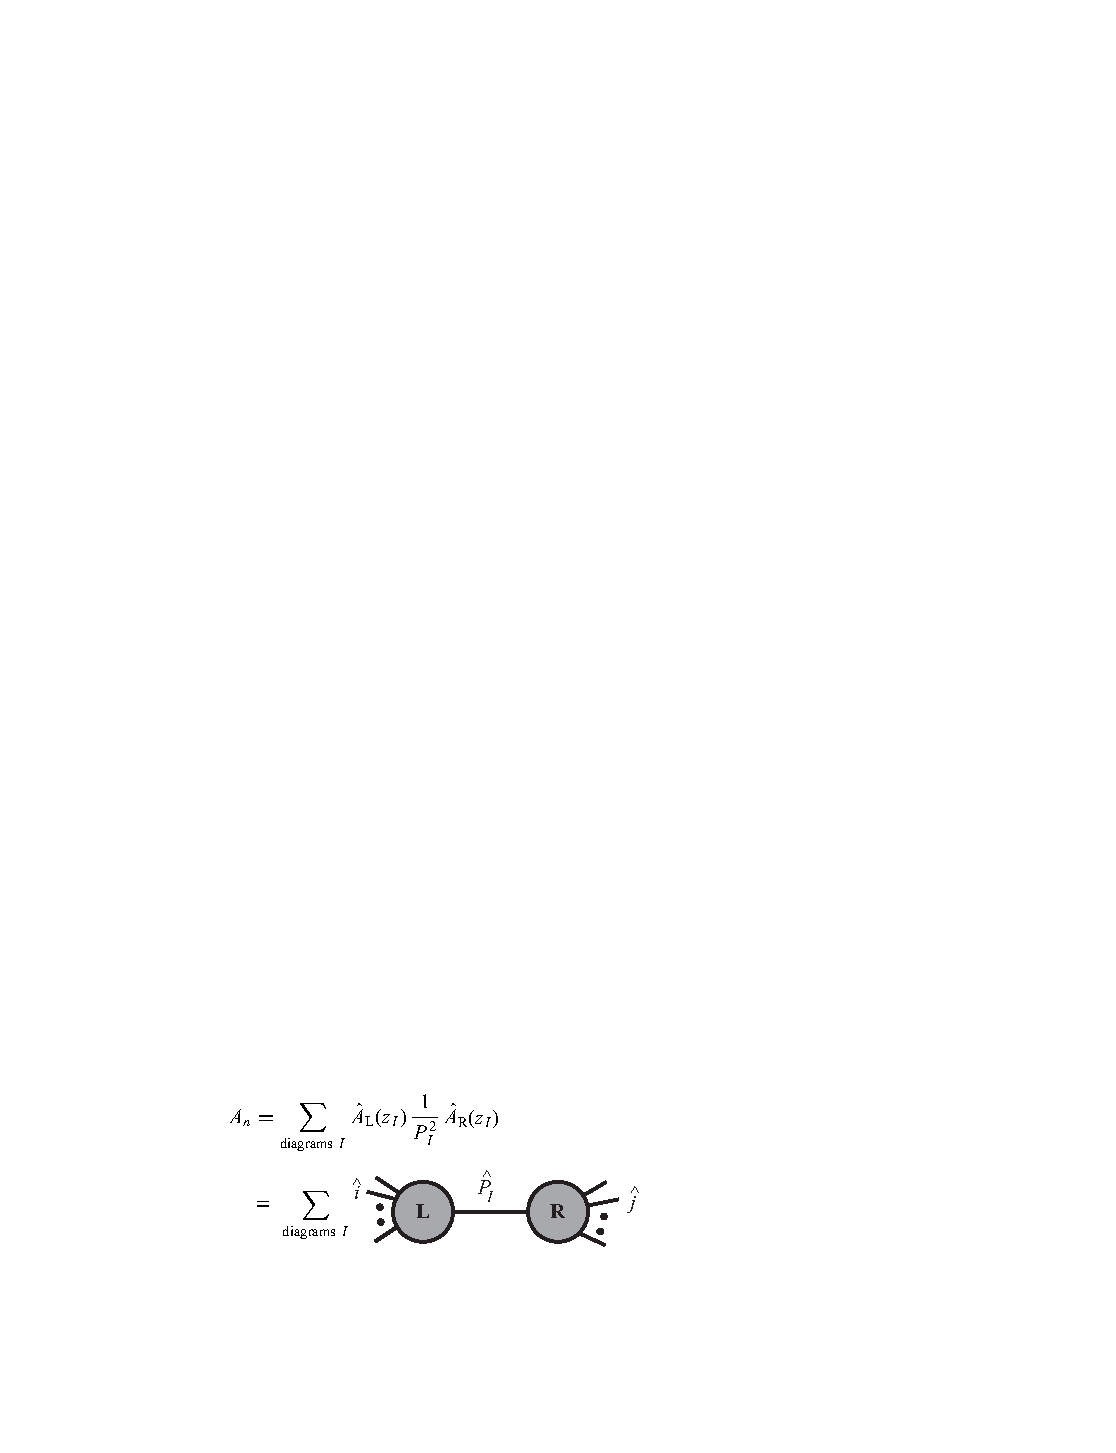
\includegraphics[width=7cm]{figs/3.pdf}
 				\caption{BCFW Recursion Relations.}
 			\end{figure}
 		\end{columns}
 	\end{frame}
	
	\begin{frame}
		\frametitle{More theories and their connections}
		\begin{columns}
			\column{0.4\textwidth}
			\begin{itemize}
				\setlength{\itemsep}{.3cm}
				\item{
					Scattering equations are very difficult to find all (n-3)! solutions. In this sense, the CHY formula doesn't bring us a new efficient tool for calculating amplitudes. But it gives us a unified framework to consider connections between different theories.
				}
			\end{itemize}
			\column{0.6\textwidth}
			\only<2>{
				\begin{figure}
					\centering
					% Requires \usepackage{graphicx}
					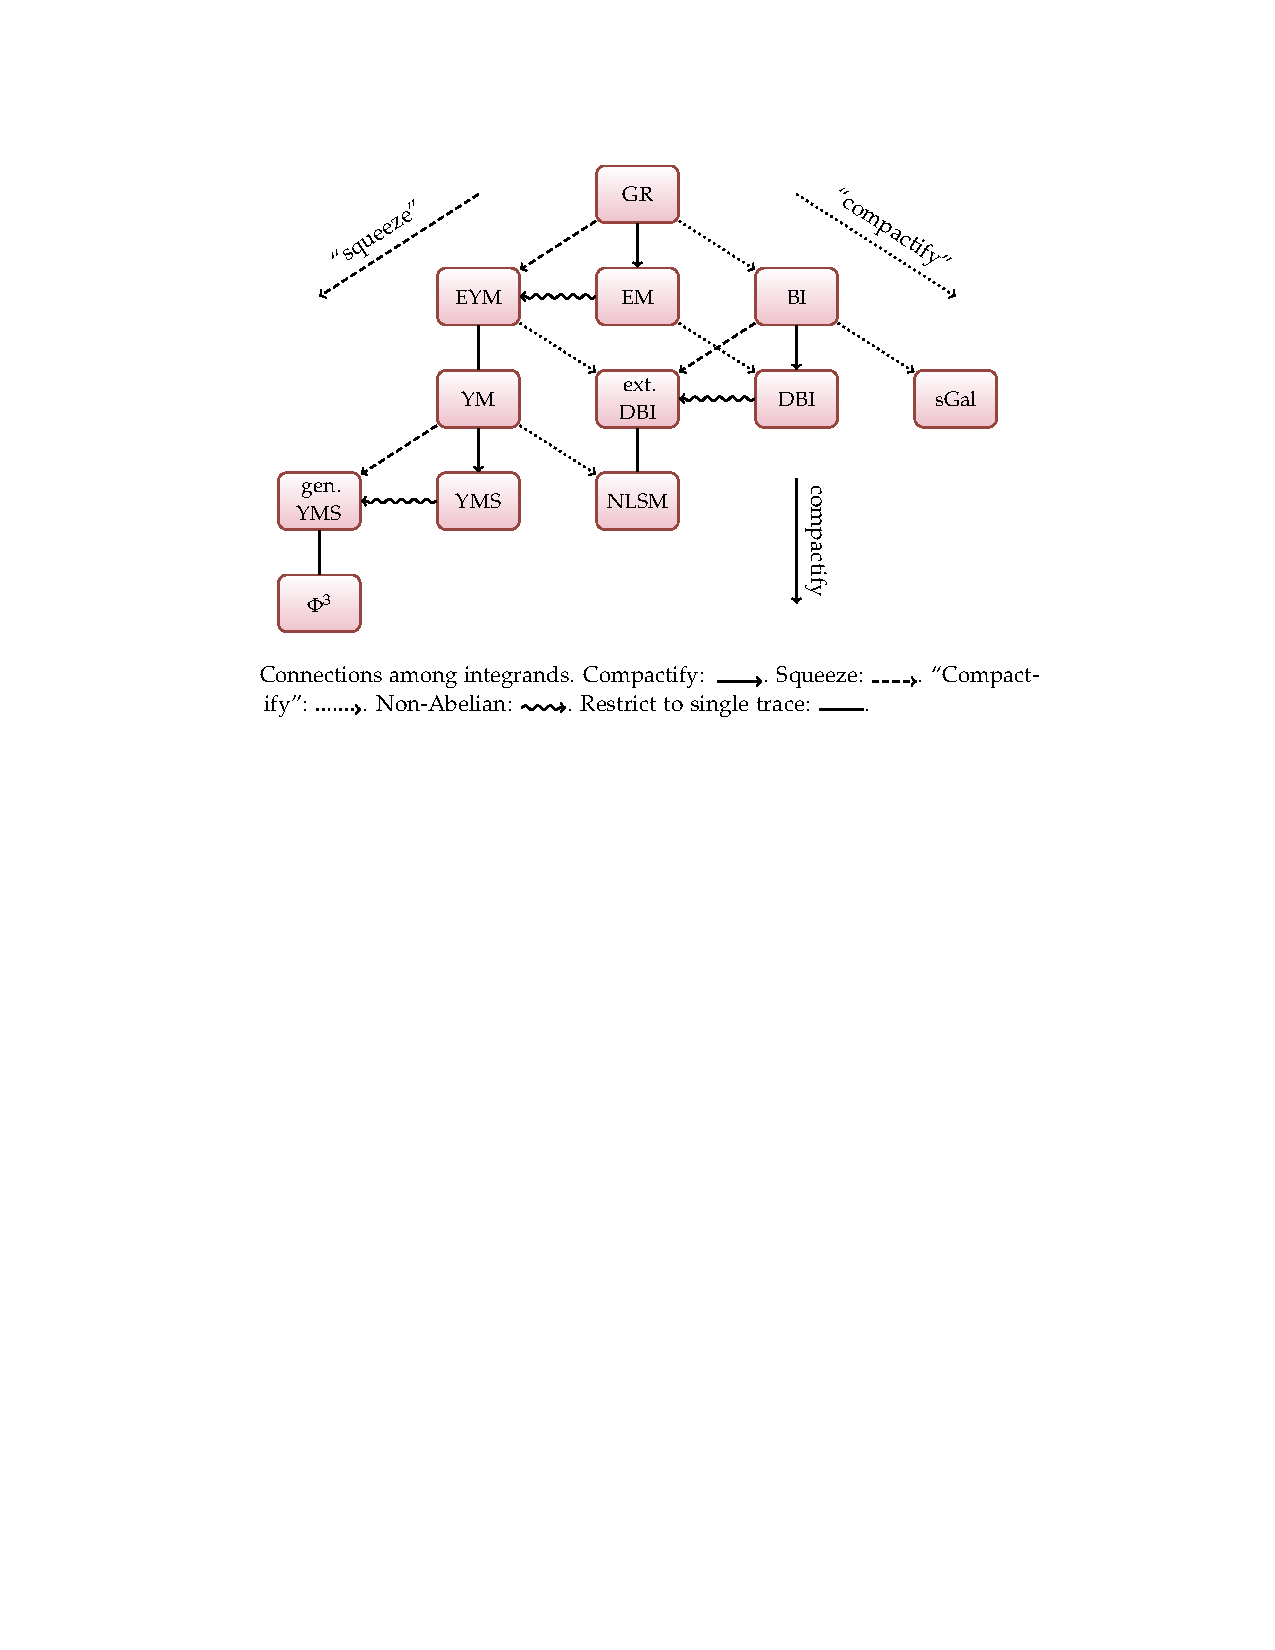
\includegraphics[width=7cm]{figs/1.pdf}
					\caption{Theory Web.}
			\end{figure}}
		\only<1>{
			\begin{figure}
				\centering
				% Requires \usepackage{graphicx}
				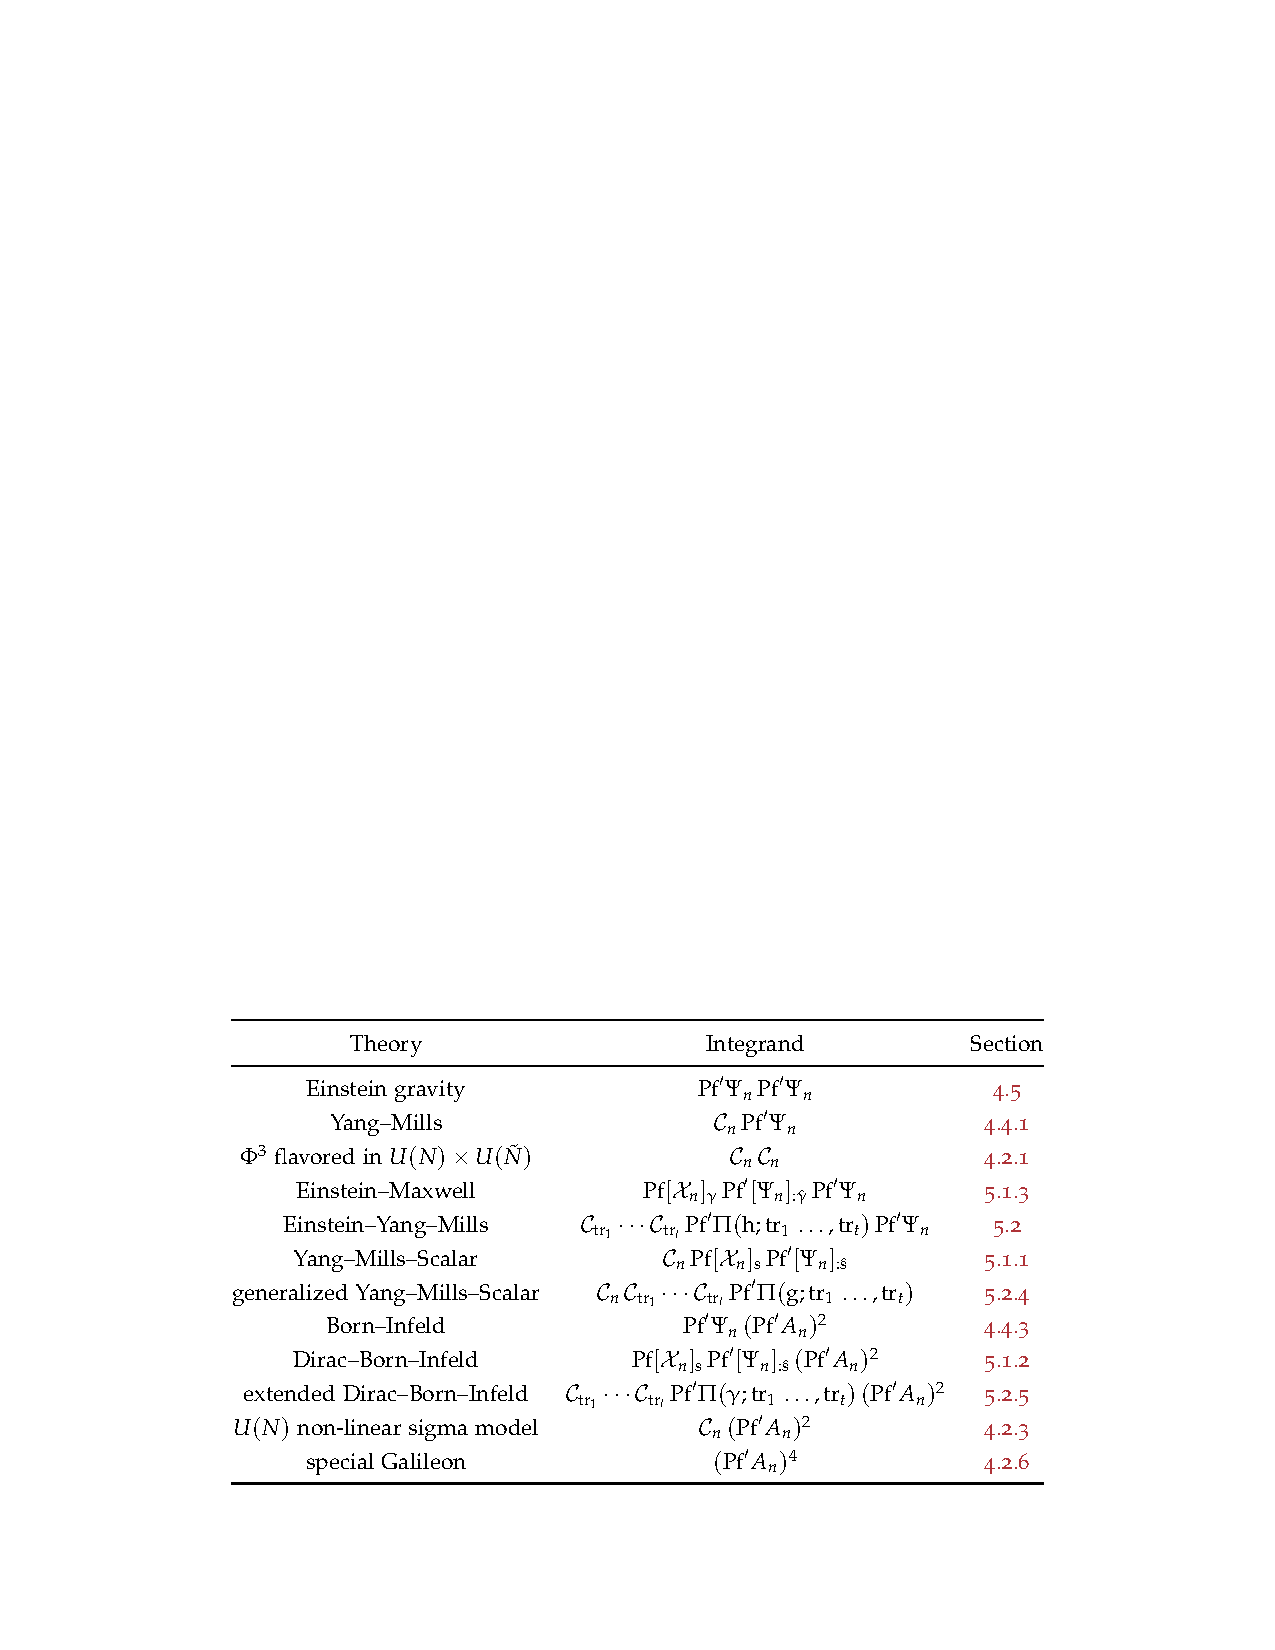
\includegraphics[width=7cm]{figs/4.pdf}
				\caption{CHY integrands of different QFTs}
			\end{figure}
		}
		\end{columns}
	\end{frame}
	
	\begin{frame}
		\frametitle{KLT double copy}
		Gravity = YM$^2$/$\phi^3$,
		\begin{equation}
			\boxed{M_n=(-1)^n\sum_{\beta,\gamma}\frac{A_n(1,\beta_{2,n-1},n)\widetilde{\mathcal{S}}[\beta_{2,n-1}|\gamma_{2,n-1}]_{p_n}\widetilde{A}_n(n,\gamma_{2,n-1},1)}{s_{23...n}}}
		\end{equation}
		Where, KLT kernel $\mathcal{S}[\alpha|\beta]$ can be constructed by double partial amplitudes of $\phi^3$ theory:
		\begin{equation}
			S[\alpha|\beta]=\prod_{i=2}^{n-2}\left(s_{1,\alpha(i)}+\sum_{j=2}^{i-1}\theta(\alpha(j),\alpha(i))_\beta s_{\alpha(j),\alpha(i)}\right)=m(\alpha|\beta)^{-1}
		\end{equation}
		So, we divide YM$^2$ by $\phi^3$.
	\end{frame}
	
	\begin{frame}
		\frametitle{KLT relation{\color{red}s}}
		KLT othogonality eq.5 can be rewrited as,
		\begin{equation}
			\delta_{\alpha,\gamma}=\sum_{\beta\in S_{n-3}}\int d\mu_n\mathbf{PT}(\alpha)\mathbf{PT}(\beta)S[\beta|\gamma]
		\end{equation}
			So if we have a theory $\mathcal{M}_n$ whose CHY integrand is $\mathcal{I}=\mathcal{I}^L\mathcal{I}^R$. Then we can define two partial amplitudes $\mathcal{M}^L_n$ and $\mathcal{M}^R_n$, whose CHY integrands are $\mathcal{I}^L$ and $\mathcal{I}^R$, respect-\\-ively.
			
		\vspace{.4em}
		Which gives a general KLT relation,\footnote{"KLT" suffix means we need a KLT kernel.}
		
		\begin{equation}
			\mathcal{M}_n=\mathcal{M}^L_n\otimes_{\text{KLT}}\mathcal{M}^R_n
		\end{equation}
		The CHY formalism enables us to gain insights that would otherwise be difficult to discern from the Lagrangian.
	\end{frame}
	\section*{Thanks}
	\begin{frame}
		\centering
		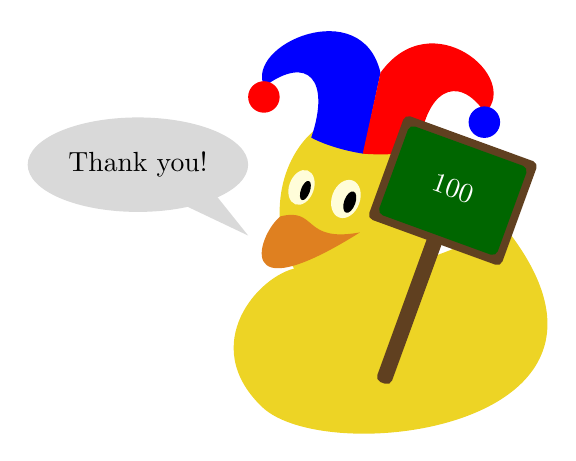
\begin{tikzpicture}[scale=2]
			\duck[harlequin=blue,niuqelrah=red,speech={Thank you!},signpost={100}]
		\end{tikzpicture}
	\end{frame} 
\end{document}